\chapter{World Model for Subgoal Planning}
\label{chap:wm-as-subgoal}
\label{chap:latent-subgoal-planning}

\section{Motivation}
\label{sec:lsp-motivation}

The previous chapters showed that a frozen world model is most useful
when it proposes short-horizon futures that are scored by a value
function trained on real data. This chapter asks whether the same
proposal-and-score pattern extends from action-level planning to
hierarchical decision making.
In standard hierarchical offline RL, the high-level policy is typically learned by behaviour cloning. It proposes subgoals that already appear in the dataset, and the low-level policy is trained to reach them. This works well but is inherently conservative. If a useful subgoal was never explicitly observed in the dataset, the high level cannot propose it, even if it would be reachable under the dynamics learned by the world model.
We therefore explore whether the world model and offline value function can be used to search over subgoals rather than merely evaluate actions. The key idea is to treat subgoals as latent states in the same space as the world model, and to rank them using long-horizon value estimates obtained by rolling out the low-level policy inside the world model. In other words, we lift the same MPC-style mechanism from action space to subgoal space.

To study this, we introduce \textbf{Latent Subgoal Planning (LSP)}. The high-level policy proposes candidate subgoals directly in the learned latent space, the world model evaluates them by simulating low-level rollouts toward each candidate, and an offline-trained value function scores the resulting outcomes. This mirrors the structure of the previous chapters, but moves the search problem one level up the hierarchy.
We adopt the hierarchical framework of HIQL-style offline goal-conditioned RL, but replace the original discrete or dataset-constrained subgoal distribution with a continuous flow-matching policy over latent subgoals and actions (see \S\ref{sec:lsp-flow}). Importantly, the core HIQL structure remains unchanged: a high-level policy proposes subgoals every $k=10$ steps, and a low-level policy executes primitive actions conditioned on those subgoals. The modification is not in the hierarchy itself, but in how the high-level proposals are generated and evaluated.
Phase~1 follows standard offline goal-conditioned HIQL training with no world model involvement. Phase~2 then attempts to improve the high-level policy using world-model rollouts and value-function scoring in the same proposal-and-score spirit as Chapter~\ref{chap:wm-planner}. The evaluation in \S\ref{sec:exp-wm-as-subgoal} tests whether this action-level pattern transfers to hierarchical subgoal spaces.

% =====================================================================
\section{Latent Subgoal Planning Architecture}
\label{sec:lsp-architecture}

The system consists of three components operating in the learned latent space $\mathcal{Z} = \mathbb{R}^{d_z}$: a value function, a high-level policy, and a low-level policy.

\paragraph{Value function.}
We use an action-free goal-conditioned value function $V(z, g)$ trained with implicit Q-learning (IQL) via expectile regression (\S\ref{sec:iql}). It is trained entirely on offline data and is never updated with world-model-generated transitions. It estimates long-horizon return from state $z$ toward goal $g$.

\paragraph{High-level policy.}
The high-level policy $\pi^{\mathrm{HL}}$ proposes a subgoal latent $w$ conditioned on the current state and task goal:
\begin{equation}
w \;\sim\; \pi^{\mathrm{HL}}(\,\cdot\mid z,\,g).
\end{equation}
Unlike standard HIQL, where subgoals are implicitly constrained to match dataset behaviour, here $w$ is a continuous latent in the same space as $z$ and $g$. This makes it directly compatible with the world model, which can evaluate candidate subgoals by simulating trajectories toward them.

\paragraph{Low-level policy.}
The low-level policy $\pi^{\mathrm{LL}}$ maps the current latent and subgoal to primitive actions:
\begin{equation}
a \;\sim\; \pi^{\mathrm{LL}}(\,\cdot\mid z,\,w).
\end{equation}
The high-level policy replans every $k=10$ steps, following the standard horizon choice used in HIQL-style hierarchical control. Between replanning steps, the low-level policy executes actions conditioned on a fixed subgoal.

\subsection{Flow-Matching High- and Low-Level Policies}
\label{sec:lsp-flow}

Both policies are parameterised as flow-matching models, following the same construction used in Chapter~\ref{chap:wm-planner}. We do not restate the full formulation here and refer instead to \S\ref{sec:lsp-architecture} and the flow policy background (\S\ref{sec:fql-bg}).
The key idea is that instead of modelling a unimodal Gaussian over subgoals or actions, the policy learns a transport map from Gaussian noise to the empirical behaviour distribution. This is particularly important in high-dimensional latent spaces such as $\mathbb{R}^{d_z}$, where behaviour is highly multi-modal and concentrated on narrow manifolds.

Training follows the standard flow-matching behaviour cloning objective. Given a target sample $x_1$ (either a subgoal $w$ or an action $a$), we interpolate between Gaussian noise $x_0 \sim \mathcal{N}(0, I)$ and the target:
\begin{equation}
x_t = (1-t)\,x_0 + t\,x_1, \qquad t \sim \mathrm{Unif}[0,1],
\end{equation}
and train a velocity field to predict the displacement:
\begin{equation}
\mathcal{L}_{\mathrm{BC}}
= \mathbb{E}\!\left[
\|u_\theta(\mathrm{cond},\,x_t,\,t) - (x_1 - x_0)\|_2^2
\right].
\label{eq:lsp-bc}
\end{equation}
At inference time, samples are generated by integrating the learned velocity field using $S$ Euler steps. In Phase~2, these generated samples are further reweighted using advantage signals derived from the value function, following the same HIQL-style idea of advantage-weighted regression.

\subsection{Offline Hierarchical Training}
\label{sec:lsp-phase1}

Phase~1 trains the full hierarchical system purely offline, without any world model interaction. The value function is trained using expectile regression (\S\ref{sec:iql}), and both policies are trained using advantage-weighted flow-matching.

For each transition, an advantage estimate is computed from the value function and used to weight the flow-BC objective:
\begin{equation}
w_t = \min\!\bigl(\exp(\alpha\,\hat{A}_t),\,100\bigr),
\qquad
\hat{A}_t = \tfrac{1}{2}\sum_{i=1}^{2}
\bigl[
V_{\phi_i}(z_{t+1}, g_{\mathrm{sub}}) - V_{\phi_i}(z_t, g_{\mathrm{sub}})
\bigr].
\end{equation}
The clipping at $100$ prevents a small number of high-advantage transitions from dominating optimisation. The resulting Phase~1 policy provides the offline hierarchical baseline used by the Phase~2 world-model updates; its performance is reported in \S\ref{sec:exp-lsp-phase1} (Table~\ref{tab:lsp-phase1}).

% =====================================================================
\section{Using World Model to Improve High-Level Policies}
\label{sec:lsp-phase2}

After Phase-1, the high-level policy has learned a strong but dataset-limited mapping from $(z,g)$ to subgoals. It proposes latents that are consistent with the dataset distribution, but cannot reliably extrapolate beyond it. Phase-2 investigates whether the world model can be used as a proposal evaluator that reshapes this distribution using imagined rollouts, without ever changing the low-level policy or the value function.
Across all experiments, the value function $V$ and the low-level policy $\pi^{\mathrm{LL}}$ are frozen at their Phase-1 parameters. Only the high-level policy $\pi^{\mathrm{HL}}$ is updated. The world model is used to evaluate a candidate subgoal $w$ by first executing the low-level controller inside the model for $k$ steps starting from the current latent $z$, as illustrated in Figure~\ref{fig:lsp-subgoal-grounding}. Concretely, the low-level policy is unrolled conditionally on $w$, and the resulting latent after $k$ steps is
\begin{equation}
z_{\mathrm{ach}} = z_k,\quad
z_{h+1} = f_\psi\!\bigl(z_h, a_h\bigr),\quad
a_h \sim \pi^{\mathrm{LL}}(\cdot \mid z_h, w),\quad
z_0 = z,\quad h=0,\dots,k-1.
\label{eq:lsp-roll}
\end{equation}
The subgoal is then evaluated by how much downstream value it produces under the frozen critic, i.e. $V(z_{\mathrm{ach}}, g)$.

\begin{figure}[t]
    \centering
    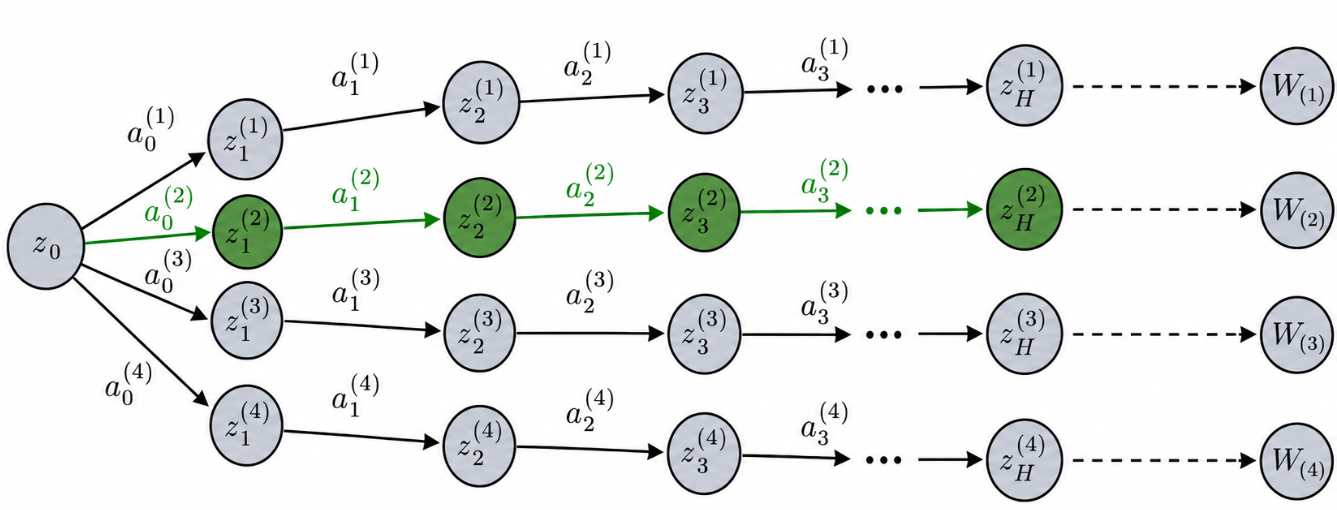
\includegraphics[width=\linewidth]{figures/subgoal_grounding.png}
    \caption{World-model-based evaluation of candidate high-level subgoals in Phase-2 of Latent Subgoal Planning. Starting from the current latent state $z_0$, the high-level policy proposes multiple candidate subgoals. For each candidate, the frozen low-level policy is rolled out for $H$ steps inside the world model, producing an imagined latent trajectory and a terminal latent $z_H^{(i)}$. Each terminal latent is then scored using the frozen value function $V$, yielding a weight or ranking for the corresponding candidate subgoal. The highest-scoring rollout indicates which subgoal is predicted to produce the greatest downstream value relative to the ultimate goal.}
    \label{fig:lsp-subgoal-grounding}
\end{figure}

The core question in all subsequent methods is whether we can use this imagined closed-loop rollout to reshape the distribution of high-level subgoals without breaking the alignment between the high- and low-level policies learned in Phase-1.

\subsection{AWR with Dataset Subgoal Targets}
\label{sec:lsp-awr-data}

The first and most direct idea is to keep the Phase-1 subgoal support fixed and simply reweight it using world-model rollouts. For each training state $z$, we sample a small set of candidate subgoals $\{w_n\}_{n=1}^N$ from the original dataset subgoal distribution used in Phase-1. Each candidate is evaluated by rolling the frozen low-level policy for $k$ steps inside the world model as in Eq.~\eqref{eq:lsp-roll}, producing $z_{\mathrm{ach},n}$.

We define an advantage relative to the current state:
\begin{equation}
J_n = V(z_{\mathrm{ach},n},\,g) - V(z,\,g),
\end{equation}
which measures whether attempting to reach $w_k$ improves predicted long-term return compared to staying at $z$. These advantages are normalised within the batch and converted into AWR weights $w_n = \min(\exp(\alpha J_n), 100)$. The high-level policy is then updated by a weighted flow-BC objective toward the dataset subgoals.

\paragraph{Distributional sharpness.}
Although this procedure is locally well-defined, it introduces a tension between the Phase-1 subgoal distribution and the broader dataset support. Phase-1 has already concentrated probability mass on a relatively narrow set of subgoals that are consistently useful under the frozen low-level policy. In contrast, the dataset distribution includes many subgoals that are valid transitions but not necessarily optimal intermediate targets.
Even with AWR weighting, every batch still contains non-zero probability mass on suboptimal subgoals. Over many updates, this can broaden the high-level flow: probability mass is pulled away from the sharp Phase-1 modes toward the wider dataset support. Increasing $\alpha$ reduces this effect but weakens the learning signal, while decreasing $\alpha$ accelerates the drift.

\subsection{AWR with On-Policy Subgoal Targets}
\label{sec:lsp-awr-self}

A natural response is to eliminate the mismatch between the dataset subgoal distribution and the current policy by sampling subgoals directly from $\pi^{\mathrm{HL}}(\cdot \mid z,g)$. This ensures that all candidates lie within the current support of the high-level policy, avoiding the broadening pressure observed above.
Each candidate subgoal $w_n \sim \pi^{\mathrm{HL}}(\cdot \mid z,g)$ is evaluated using the same world-model rollout procedure in Eq.~\eqref{eq:lsp-roll}, and scored by $V(z_{\mathrm{ach},n}, g)$. These scores are again converted into AWR weights and used to update the flow policy.

\paragraph{Value miscalibration risk.}
This variant exposes a different failure mode: the frozen value function $V(z,g)$ is not trained to evaluate arbitrary latent subgoals $w$, but only dataset-induced states. In particular, it assigns high value to latents that are close to the goal $g$, even if they are not actually reachable from $z$ within $k$ low-level steps.
As training progresses, the high-level policy exploits this bias by shifting probability mass toward subgoals $w \approx g$. However, when these subgoals are executed through the frozen low-level policy inside the world model, the resulting $z_{\mathrm{ach}}$ remains far from $g$, leading to low realised value $V(z_{\mathrm{ach}}, g)$. This creates a systematic disconnect between the training signal $V(w,g)$ and the true outcome of executing $w$ via the low-level controller, resulting in instability rather than improvement.

\subsection{AWR with Achieved Latent States}
\label{sec:lsp-hrf}

To remove the mismatch between proposed subgoals and executed outcomes, we replace the training target with the \emph{achieved state} of the rollout. Instead of regressing the high-level policy toward the proposed subgoal $w$, we regress it toward the actually reached latent $z_{\mathrm{ach}}$ obtained after executing $\pi^{\mathrm{LL}}$ in the world model for $k$ steps.

The resulting objective is:
\begin{equation}
\mathcal{L}_{\mathrm{HRF}} = \mathbb{E}\!\left[
w_n\cdot\mathcal{L}_{\mathrm{BC}}^{\mathrm{per\text{-}sample}}
\!\bigl(\pi^{\mathrm{HL}},\,z_{\mathrm{ach},n}\bigr)\right],
\quad
w_n = \min\!\bigl(\exp(\alpha\cdot\hat J_n),\,100\bigr),
\quad
J_n = V(z_{\mathrm{ach},n},\,g) - V(z,\,g).
\end{equation}
This ensures that learning is grounded in what the low-level policy can actually achieve under the world model, rather than what the high-level policy proposes.

\paragraph{Distributional mismatch between levels.}
Despite being more consistent, this objective changes the effective training distribution of the high-level policy. In Phase-1, $\pi^{\mathrm{HL}}$ is trained to produce subgoals drawn from a dataset-aligned distribution $\mathcal{D}_w$, which is itself matched to what $\pi^{\mathrm{LL}}$ expects as conditioning input.
Under HRF, the high-level policy is instead trained toward $z_{\mathrm{ach}}$, which lies in a different region of latent space: it reflects what the frozen low-level policy can reach in $k$ steps starting from $z$, not what appears as intermediate subgoals in the dataset. Although both lie in $\mathbb{R}^{d_z}$, their distributions are not aligned.
As a result, the high-level policy gradually shifts away from $\mathcal{D}_w$. The low-level policy, which has not been updated, begins to receive subgoal inputs outside its training distribution, making execution quality increasingly fragile despite the improved internal consistency of the training signal.

\paragraph{Summary of Phase-2.}
Quantitative results for the Phase-2 updates are reported in
\S\ref{sec:exp-phase2-awr} (Table~\ref{tab:lsp-phase2-awr}) and
\S\ref{sec:exp-phase2-hrf} (Table~\ref{tab:lsp-hrf}), with further
ablations in Appendix~\ref{app:lsp-ablations}. The shared distributional
risk is analysed next.

\section{High--Low Level Policy Coupling Failure Mode}
\label{sec:lsp-barrier}

The central risk in Phase~2 is not only model error or value noise, but a structural constraint of the hierarchical decomposition itself: the high-level policy $\pi^{\mathrm{HL}}$ and low-level policy $\pi^{\mathrm{LL}}$ are co-adapted in Phase~1, and their compatibility depends on a shared implicit distribution over subgoals. Any update that changes this distribution without simultaneously re-establishing that compatibility can break the equilibrium.

The three approaches can be grouped according to how they violate this constraint. Updating with dataset subgoals (Approach 1) pushes the high-level policy toward the broader dataset marginal, away from the concentrated subgoal distribution that the low-level has learned to execute reliably. Updating with on-policy subgoals preferences (Approach 2) does not change the support as drastically, but instead shifts probability mass toward near-goal or high-value regions that are not necessarily reachable within $k$ steps under the frozen low-level controller. Hindsight reality forcing (Approach 3) goes further and replaces the target distribution entirely with achieved latents $z_{\mathrm{ach}}$, which are by construction tied to the current low-level dynamics inside the world model. In each case, the effective conditioning distribution seen by $\pi^{\mathrm{LL}}$ can drift away from the one it was trained on.

A useful diagnostic is to remove the world model from the advantage computation entirely. In this controlled ablation, WM-evaluated advantages are replaced with
$V(w_k, g) - V(z, g)$ computed directly from the frozen critic, while the dataset-subgoal AWR update is otherwise unchanged. This isolates whether the central issue is compounding model error or the mismatch between the subgoal distribution induced by Phase-2 updates and the distribution on which the hierarchical policies were jointly trained. The world model can make this mismatch explicit, but it is not the only possible source of the mismatch.

\paragraph{Jointly updating the hierarchy.}
A natural repair is to update both levels so that the low-level policy can track the evolving subgoal distribution induced by the high-level updates. We evaluate this directly by allowing $\pi^{\mathrm{LL}}$ to train under the same WM-derived supervision as $\pi^{\mathrm{HL}}$. This ablation tests whether distributional drift can be absorbed by the hierarchy itself, or whether moving both policies simply shifts the inconsistency to the value function and remaining offline anchors, which still reflect the original Phase-1 equilibrium.

The underlying risk mirrors the moving-target problem analysed in Chapter~\ref{chap:mpc-distillation}. Here, the analogue is the frozen value function and the jointly trained policies: once one part of the system shifts its effective data distribution, the others can only remain consistent by shifting as well. We therefore conjecture that successful joint optimisation would require either (i) a value function that tracks the evolving hierarchy, or (ii) a mechanism that constrains both levels to a shared, fixed subgoal distribution throughout training. We leave both directions as future work.

\section{Summary}
This chapter defined a hierarchical extension of the proposal-and-score
pattern used in action-level planning. As argued in
\S\ref{sec:lsp-barrier}, the key methodological issue is the coupling
between the high-level subgoal distribution and the low-level policy
trained to execute it. Improving the high level therefore requires
maintaining that compatibility, not only finding higher-valued candidate
subgoals.
